\documentclass[10pt,landscape,a4paper]{article}
\usepackage[utf8]{inputenc}
\usepackage[ngerman]{babel}
\usepackage{tikz}
\usetikzlibrary{shapes,positioning,arrows,fit,calc,graphs,graphs.standard}
\usepackage[nosf]{kpfonts}
\usepackage[t1]{sourcesanspro}
%\usepackage[lf]{MyriadPro}
%\usepackage[lf,minionint]{MinionPro}
\usepackage{multicol}
\usepackage{wrapfig}
\usepackage[top=0mm,bottom=1mm,left=0mm,right=1mm]{geometry}
\usepackage[framemethod=tikz]{mdframed}
\usepackage{microtype}
\usepackage{amsmath}

\let\bar\overline

\definecolor{myblue}{cmyk}{1,.72,0,.38}
\definecolor{forestgreen}{RGB}{34,139,34}

\def\firstcircle{(0,0) circle (1.5cm)}
\def\secondcircle{(0:2cm) circle (1.5cm)}

\colorlet{circle edge}{myblue}
\colorlet{circle area}{myblue!5}

\tikzset{filled/.style={fill=circle area, draw=circle edge, thick},
    outline/.style={draw=circle edge, thick}}

\pgfdeclarelayer{background}
\pgfsetlayers{background,main}

\everymath\expandafter{\the\everymath \color{myblue}}
\everydisplay\expandafter{\the\everydisplay \color{myblue}}

\renewcommand{\baselinestretch}{.8}
\pagestyle{empty}

\global\mdfdefinestyle{header}{%
linecolor=gray,linewidth=1pt,%
leftmargin=0mm,rightmargin=0mm,skipbelow=0mm,skipabove=0mm,
}

\newcommand{\header}{
\begin{mdframed}[style=header]
\footnotesize
\sffamily
Cheat sheet\\
by~Wei~Wu,~page~\thepage~of~2
\end{mdframed}
}

\makeatletter
\renewcommand{\section}{\@startsection{section}{1}{0mm}%
                                {.2ex}%
                                {.2ex}%x
                                {\color{myblue}\sffamily\small\bfseries}}
\renewcommand{\subsection}{\@startsection{subsection}{1}{0mm}%
                                {.2ex}%
                                {.2ex}%x
                                {\sffamily\bfseries}}



\def\multi@column@out{%
   \ifnum\outputpenalty <-\@M
   \speci@ls \else
   \ifvoid\colbreak@box\else
     \mult@info\@ne{Re-adding forced
               break(s) for splitting}%
     \setbox\@cclv\vbox{%
        \unvbox\colbreak@box
        \penalty-\@Mv\unvbox\@cclv}%
   \fi
   \splittopskip\topskip
   \splitmaxdepth\maxdepth
   \dimen@\@colroom
   \divide\skip\footins\col@number
   \ifvoid\footins \else
      \leave@mult@footins
   \fi
   \let\ifshr@kingsaved\ifshr@king
   \ifvbox \@kludgeins
     \advance \dimen@ -\ht\@kludgeins
     \ifdim \wd\@kludgeins>\z@
        \shr@nkingtrue
     \fi
   \fi
   \process@cols\mult@gfirstbox{%
%%%%% START CHANGE
\ifnum\count@=\numexpr\mult@rightbox+2\relax
          \setbox\count@\vsplit\@cclv to \dimexpr \dimen@-1cm\relax
\setbox\count@\vbox to \dimen@{\vbox to 1cm{\header}\unvbox\count@\vss}%
\else
      \setbox\count@\vsplit\@cclv to \dimen@
\fi
%%%%% END CHANGE
            \set@keptmarks
            \setbox\count@
                 \vbox to\dimen@
                  {\unvbox\count@
                   \remove@discardable@items
                   \ifshr@nking\vfill\fi}%
           }%
   \setbox\mult@rightbox
       \vsplit\@cclv to\dimen@
   \set@keptmarks
   \setbox\mult@rightbox\vbox to\dimen@
          {\unvbox\mult@rightbox
           \remove@discardable@items
           \ifshr@nking\vfill\fi}%
   \let\ifshr@king\ifshr@kingsaved
   \ifvoid\@cclv \else
       \unvbox\@cclv
       \ifnum\outputpenalty=\@M
       \else
          \penalty\outputpenalty
       \fi
       \ifvoid\footins\else
         \PackageWarning{multicol}%
          {I moved some lines to
           the next page.\MessageBreak
           Footnotes on page
           \thepage\space might be wrong}%
       \fi
       \ifnum \c@tracingmulticols>\thr@@
                    \hrule\allowbreak \fi
   \fi
   \ifx\@empty\kept@firstmark
      \let\firstmark\kept@topmark
      \let\botmark\kept@topmark
   \else
      \let\firstmark\kept@firstmark
      \let\botmark\kept@botmark
   \fi
   \let\topmark\kept@topmark
   \mult@info\tw@
        {Use kept top mark:\MessageBreak
          \meaning\kept@topmark
         \MessageBreak
         Use kept first mark:\MessageBreak
          \meaning\kept@firstmark
        \MessageBreak
         Use kept bot mark:\MessageBreak
          \meaning\kept@botmark
        \MessageBreak
         Produce first mark:\MessageBreak
          \meaning\firstmark
        \MessageBreak
        Produce bot mark:\MessageBreak
          \meaning\botmark
         \@gobbletwo}%
   \setbox\@cclv\vbox{\unvbox\partial@page
                      \page@sofar}%
   \@makecol\@outputpage
     \global\let\kept@topmark\botmark
     \global\let\kept@firstmark\@empty
     \global\let\kept@botmark\@empty
     \mult@info\tw@
        {(Re)Init top mark:\MessageBreak
         \meaning\kept@topmark
         \@gobbletwo}%
   \global\@colroom\@colht
   \global \@mparbottom \z@
   \process@deferreds
   \@whilesw\if@fcolmade\fi{\@outputpage
      \global\@colroom\@colht
      \process@deferreds}%
   \mult@info\@ne
     {Colroom:\MessageBreak
      \the\@colht\space
              after float space removed
              = \the\@colroom \@gobble}%
    \set@mult@vsize \global
  \fi}

\makeatother
\setlength{\parindent}{0pt}

\begin{document}
\small
\begin{multicols*}{5}
	\section{Mathematical Basic}
\subsection*{Identities and Inequalities}
Binomial expansion theorem:\\
$(x+y)^n=\sum_{i=0}^{n}\binom{n}{i}x^i y^{n-i}$\\
Proposition:\\
\begin{itemize}
    \item For all $x\ge 1$ it holds that $(1-1/x)^x\le e^{-1}$
    \item For all $x$ it holds that $1-x\le e^{-x}$
    \item For all $x$ with $0\le x \le 1$ it holds that
\end{itemize}
$e^{-x}\le 1-(1-\frac{1}{e})\cdot x\le 1-\frac{x}{2}$\\
\subsection*{Asymptotic Notation}
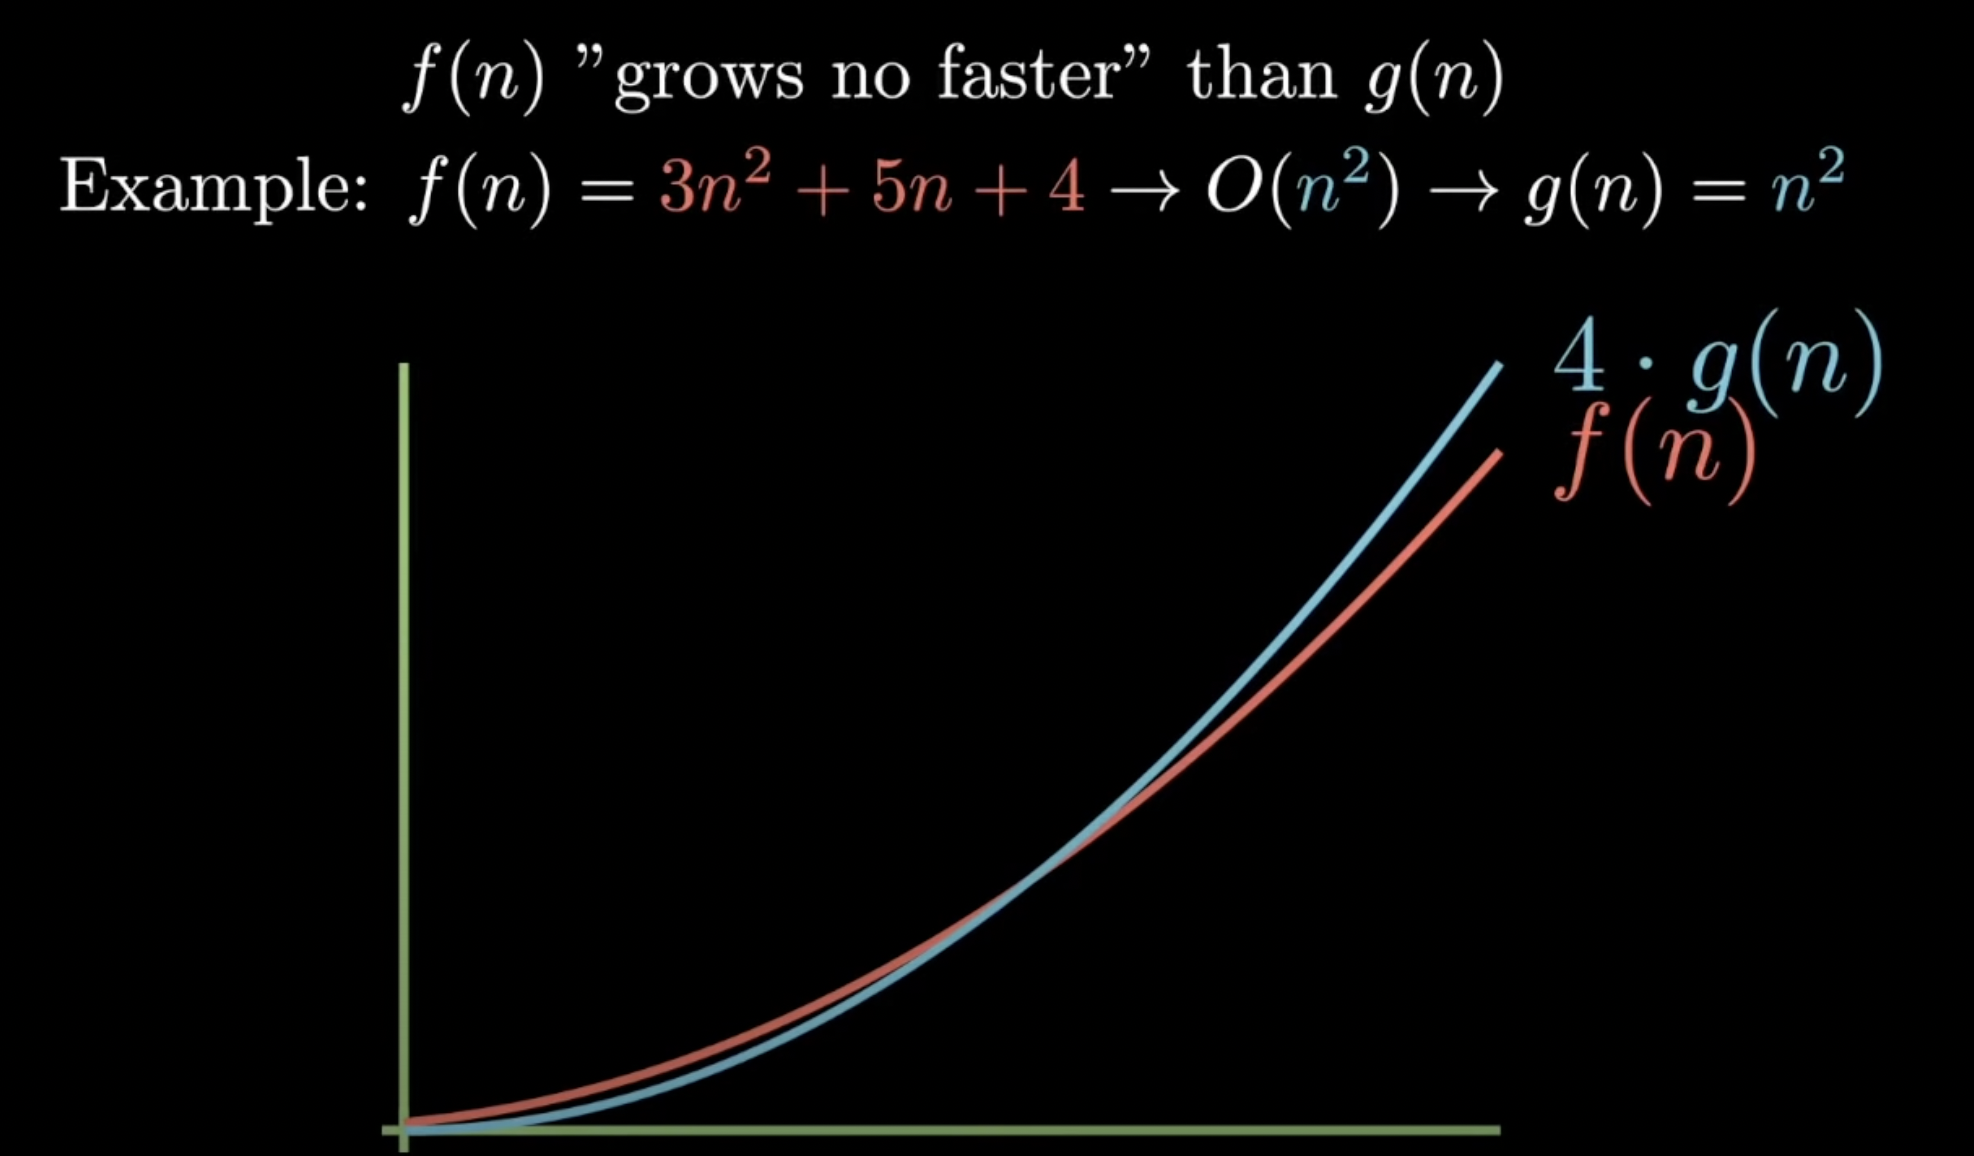
\includegraphics[width=\columnwidth]{big-o-explained.png}
Let $f(n),g(n)$ be functions from non-negative integers to non-negative reals. 
Then:
\begin{itemize}
    \item $f(n)=\mathcal{O}(g(n))$ means that there exist positive integers c 
    and n' such that for all $n > n'$ it holds that $f(n)\le c \cdot g(n)$
    \item $f(n)=\varOmega (g(n))$ means that there exist positive integers c
    and n' such that for all $n > n'$ it holds that $f(n)\ge c\cdot g(n)$.
    \item $f(n)=\varTheta (g(n))$ means that there exist positive integers 
    $c_{1}$ and $c_{2}$ such that for all $n > n'$ it holds that 
    $c_{1}\cdot g(n) \le f(n) \le c_{2} \cdot g(n)$
    \item $f(n)=o(g(n))$ means that $\lim_{n \to \infty} \frac{f(n)}{g(n)}=0$ 
    \item $f(n)=\omega (g(n))$ means that 
    $\lim_{n \to \infty} \frac{f(n)}{g(n)}=\infty$ 
\end{itemize}

\subsection*{Basic Probability}

By definition:\\
$\Pr[E] = 1 - \Pr[\bar{E}]$\\
$\Pr[E_1\wedge E_2]\le \Pr[E_1]$\\
$\Pr[E_1 \vee E_2]\ge\Pr[E_1]$\\
When $E_1$ $E_2$ are independent:\\
$\Pr[E_1\wedge E_2]=\Pr[E_1] \cdot \Pr[E_2]$\\
Union Bound:\\
$\Pr[E_1\vee E_2]\le\Pr[E_1]+\Pr[E_2]$\\
Bayes' Theorem:\\
$\Pr[E_1|E_2] = \frac{\Pr[E_2|E_1]\cdot\Pr[E_1]}{\Pr[E_2]}$\\
Let $E_1,\cdots ,E_n$ be events such that $Pr[E_1\vee\cdots E_n]=1$ and 
$\Pr[E_i\wedge E_j]=0$ for all $i\neq j$. That is, the ${E_i}$ \emph{partition} 
the space of all possible events, so that with probability 1 exactly one of the
events $E_i$ occurs. Then for any F:\\
$\Pr[F]=\sum_{i=1}^{n}\Pr[F\wedge E_i]$\\
when $n=2$ and $E_2=\bar{E}_1$, giving:\\
$\Pr[F]=\Pr[F|E_1]\cdot\Pr[E_1]+\Pr[F|\bar{E}_1]\cdot\Pr[\bar{E}_1]$\\
we get a tighter union bound:\\
$\Pr[E_1\vee E_2]\le\Pr[E_1]+\Pr[E_2|\bar{E}_1]$\\
$\Pr[\vee^{k}_{i=1}E_{i}]
\le\Pr[E_1]+\sum^{k}_{i=2}\Pr[E_i|\bar{E}_1\wedge\cdots\wedge\bar{E}_{i-1}]$\\
   \section{Perfectly Secret Encryption}

\subsection*{Definition}
key: $k \in \mathcal{K}$ The distribution over $\mathcal{K}$ is 
the one defined by running $Gen$ and taking the output.\\
message: $m \in \mathcal{M}$\\
$c\leftarrow Enc_k(m)$: 
possibly probabilistic process by which 
message m is encrypted using key $k$ to give ciphertext $c$\\
$x \leftarrow S$: uniform selection of $x$ from a set $S$\\
$\mathcal{C}$: set of all possible ciphertexts 
that can be output by $Enc_k(m)$\\\\
let $K$ be a random variable denoting the value of the key output by $Gen$:
for any $k \in \mathcal{K},\ \Pr[K=k]$ denotes the probability that key output
by $Gen$ is equal to $k$\\\\
let $M$ be a random variable denoting the message being encrypted:
$\Pr[M=m]$ denotes the probability that the message takes on the value
$m \in \mathcal{M}$\\\\
$\ast\ $The probability distribution of the message is not 
determined by the encryption scheme itself, but instead reflects the likelihood
 of different messages being sent by the parties using the scheme, as well as an
 adversary’s uncertainty about what will be sent.\\
 $\ast\ $ $K$ and $M$ are assumed to be independent.\\\\
 Fixing an encryption scheme and a distribution over $\mathcal{M}$ determines a
 distribution over the space of ciphertexts $\mathcal{C}$ given by choosing
  a key $k \in \mathcal{K}$ and a message $m \in \mathcal{M}$, and then 
  computing the ciphertext $c \leftarrow Enc_k(m)$. Let $C$ be the random 
  variable denoting the resulting ciphertext and so, for $c \in \mathcal{C}$,
  $\Pr[C=c]$ denote the probability that the ciphertext is equal to the 
  fixed value $c$

\subsection*{Perfect secrecy} 
ciphertext should have \emph{no effect} on the adversary’s 
knowledge regarding the actual message that was sent\\
Definition: \emph{An encryption scheme 
\emph{(Gen,Enc,Dec)} with message space $\mathcal{M}$ is perfectly secret 
if for every probability distribution over $\mathcal{M}$, 
every message $m \in \mathcal{M}$, and every 
ciphertext $c \in \mathcal{C}$ for which $\Pr[C = c] > 0$:}
$\Pr[M=m|C=c]=Pr[M=m]$\\
\end{multicols*}
\end{document}